% Add only missing displacement arrowheads to the user's left-leg drawing.
% The original handwritten panel is embedded unchanged as vector PDF artwork.
% Coordinates are PDF points measured from the panel's upper-left corner.
\documentclass[border=0pt]{standalone}
\usepackage{graphicx,tikz}
\usetikzlibrary{arrows.meta}
\definecolor{handA}{RGB}{245,154,35}
\definecolor{handD}{RGB}{130,33,139}
\begin{document}
\begin{tikzpicture}[x=1bp,y=-1bp,
    displacement/.style={line width=.9bp,-{Stealth[length=3.3bp,width=2.6bp]}}]
\path[use as bounding box] (0,0) rectangle (255,385);
\begin{scope}[overlay]
\node[anchor=north west,inner sep=0] at (0,0)
  {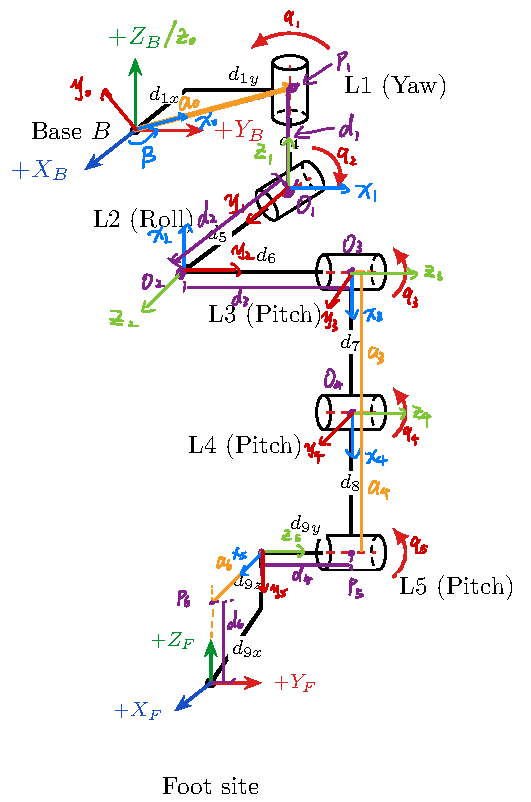
\includegraphics[width=255bp]{../assets/dh_left_handdrawn.pdf}};
% Existing handwritten a0, d1 and d2 arrowheads are already present.
% Add short arrow-ended segments on the six existing dimension strokes.
% d3: O2 -> O3, rightward, on the user's offset dimension line.
\draw[displacement,handD] (160.4,138.2)--(167.5,138.2);
% a3: O3 -> O4; a4: O4 -> P5, both downward.
\draw[displacement,handA] (173.6,191.0)--(173.6,198.0);
\draw[displacement,handA] (173.6,258.4)--(173.6,265.4);
% d5: P5 -> O5, leftward. Preserve the user's handwritten label.
\draw[displacement,handD] (134.7,271.2)--(127.5,271.2);
% a5: O5 -> P6, down-left. Preserve the user's handwritten label.
\draw[displacement,handA] (107.4,284.0)--(102.0,289.4);
% d6: P6 -> O6, downward on the user's offset dimension line.
\draw[displacement,handD] (107.2,320.6)--(107.2,327.8);
\end{scope}
\end{tikzpicture}
\end{document}
